\section{Simulations of the Reflectivity Map: Smooth, Rough, and Lipschitz Profiles}
\label{Sec: Simulations of the Reflectivity Map: TM Mode with Smooth, Rough, and Lipschitz Profiles}

We then simulated $R$ with the first frequency/wavelength range in $(6.3)$
with TM polarization and selected two--dimensional domains whose upper boundaries are shaped by the profiles
\begin{subequations}
\begin{align}
 f_{s_1}(x) &= \frac{\cos(4x)}{4}, \\
 f_{s_2}(x) &= \frac{\operatorname{exp}\left(\cos(3x)\right)}{3} - c_0,\\   
 f_r(x)&=\left(2\times 10^{-4}\right)x^4\left(2\pi - x^4\right)-c_1,\\
 f_L(x)&= \begin{cases} 
      -2x/\pi + 1, & 0 \leq x\leq \pi, \\
      2x/\pi - 3, & \pi \leq x\leq 2\pi, \\
   \end{cases}
\end{align}
\end{subequations}
where $f_{s_1},f_{s_2}$ represent a smooth $(C^{\infty})$ boundary and $f_r,f_L$ depict moderately smooth ($C^4$) and Lipschitz boundaries. Following \cite{NichollsReitich00a}, the constant $c_0$ in $(6.22\text{b})$ is chosen so that $f_{s_2}$ has zero mean (as does $f_r$ with the appropriate choice of $c_1$). The Fourier series representation of $f_r$ and $f_L$ are
\begin{subequations}
\begin{align}
f_r(x) &= \sum_{k=1}^{\infty}\frac{96\left(2k^2\pi^2 - 21\right)}{125k^8}\cos(kx),\\
f_L(x) &= \sum_{k=1}^{\infty}\frac {8}{\pi^2(2k-1)^2}\cos\big((2k-1)x\big),
\end{align}
\end{subequations}
and to minimize the effect of aliasing errors we approximated $f_r$ and $f_L$ by the truncated Fourier series
\begin{subequations}
\begin{align}
f_{r,P}(x) &= \sum_{k=1}^{P}\frac{96\left(2k^2\pi^2 - 21\right)}{125k^8}\cos(kx),\\
f_{L,P}(x) &= \sum_{k=1}^{P/2}\frac {8}{\pi^2(2k-1)^2}\cos\big((2k-1)x\big).
\end{align}
\end{subequations}
If $P \ll N_x/2$ then the effects of aliasing are minimal and we chose $P=120$ for all of our simulations. For the smooth profiles, we selected
\be
f(x)= f_{s_1}(x),
\quad
\varepsilon_{\text{max}} = 4.0, \quad
a=10,
\quad 
b=-10,
\ee
and
\be
f(x)= f_{s_2}(x),
\quad
\varepsilon_{\text{max}} = 2.0, \quad
a=4,
\quad 
b=-4,
\ee
with the parameters
\be
\alpha=0,
~~
\sigma=0.99,
~~
n^u=1,
~~
n^w = 1.1,
~~ N_x = 256,
~~ N_z = 128,
~~
N=M=20.
\ee
In Figures $26(\text{a})$ and $27(\text{a})$ we plot a single subset of the Reflectivity Map on a coordinate axis and in
Figures $26(\text{b})$ and $27(\text{b})$ we plot the Energy Defect. 
\vspace{-18mm}
\begin{figure}[H]
    \centering
    \subfloat[\centering Reflectivity Map]
    {{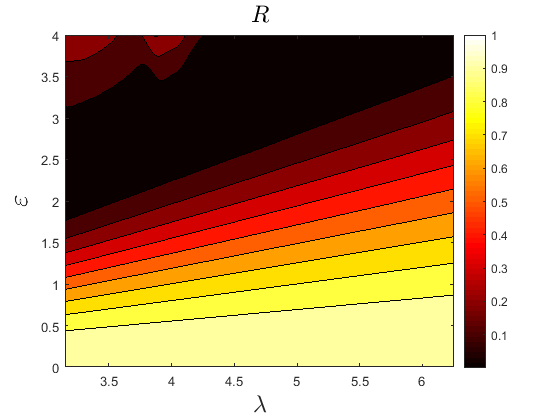
\includegraphics[width=7.6cm]{sections/6_scattering_and_reflectivity/refl_map_smooth.png} }}
    \subfloat[\centering Energy Defect]
    {{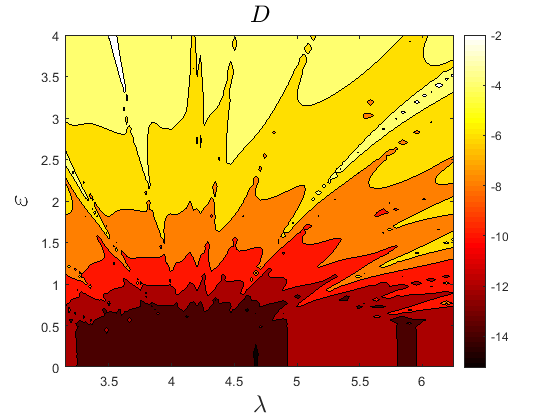
\includegraphics[width=7.6cm]{sections/6_scattering_and_reflectivity/energy_defect_smooth.png} }}
    \vspace{2mm}
    \caption{The Reflectivity Map, $R(\varepsilon,\delta)$, and Energy Defect $D$
    computed with Pad\'e summation. We set $N=M=20$ 
    with a granularity of $N_{\varepsilon}=N_{\delta}=100$ per invocation. The grating surface was $(6.25)$ and physical parameters were $(6.27)$.}
    \label{Fig:RM:Single Case 2}
\end{figure}
\vspace{-38mm}
\begin{figure}[H]
    \centering
    \subfloat[\centering Reflectivity Map]
    {{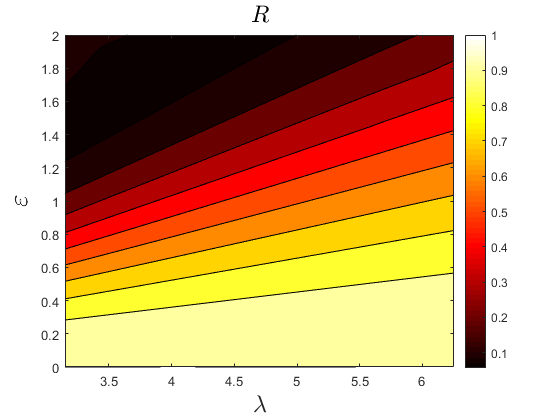
\includegraphics[width=7.6cm]{sections/6_scattering_and_reflectivity/refl_map_exp_cos_3x.png} }}
    \subfloat[\centering Energy Defect]
    {{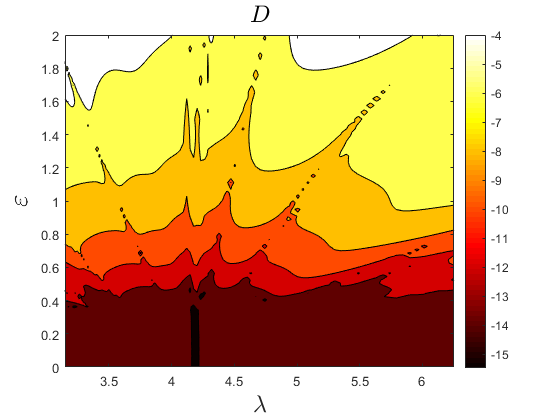
\includegraphics[width=7.6cm]{sections/6_scattering_and_reflectivity/energy_defect_exp_cos_3x.png} }}
    \vspace{2mm}
    \caption{The Reflectivity Map, $R(\varepsilon,\delta)$, and Energy Defect $D$
    computed with Pad\'e summation. We set $N=M=20$ 
    with a granularity of $N_{\varepsilon}=N_{\delta}=100$ per invocation. The grating surface was $(6.26)$ and physical parameters were $(6.27)$.}
    \label{Fig:RM:Single Case 2}
\end{figure}
\vspace{-14mm}
\hspace{-6mm}Next, for the rough profile, we selected
\be
f(x)= f_{r,P}(x),
\quad
\varepsilon_{\text{max}} = 2.0,
\quad
a = 4,
\quad
b = -4,
\ee
and for the Lipschitz profile, we selected
\be
f(x)= f_{L,P}(x),
\quad
\varepsilon_{\text{max}} = 2.0,
\quad
a=4,
\quad
b=-4,
\ee
with the parameters
\be
\alpha=0,
~~
\sigma=0.99,
~~
n^u=1,
~~
n^w = 1.1,
~~ N_x = 1024,
~~ N_z = 128,
~~
N=M=20.
\ee
In Figures $28(\text{a})$ and  $28(\text{b})$ we plot the Reflectivity Map and Energy Defect for the rough profile on a single coordinate axis and compare this to an equivalent simulation for the Lipschitz profile in Figures $28(\text{c})$ and  $28(\text{d})$.
\vspace{-17mm}
\begin{figure}[H]
    \centering
    \subfloat[\centering Reflectivity Map]
    {{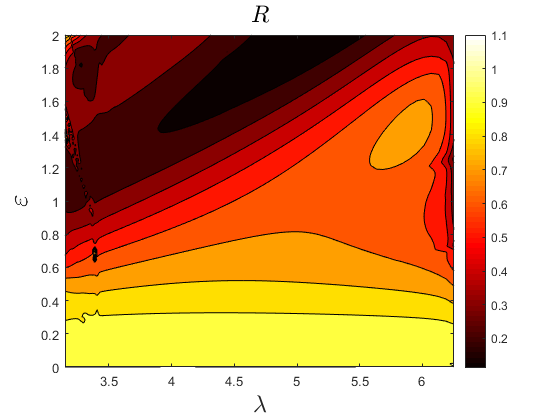
\includegraphics[width=7.6cm]{sections/6_scattering_and_reflectivity/refl_map_rough.png} }}
    \subfloat[\centering Energy Defect]
    {{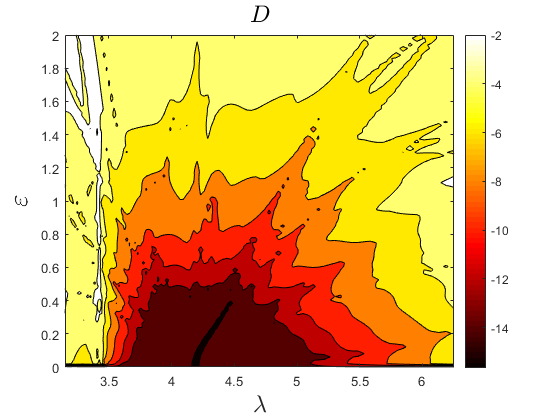
\includegraphics[width=7.6cm]{sections/6_scattering_and_reflectivity/energy_defect_rough.png} }}
    \\
    \subfloat[\centering Reflectivity Map]
    {{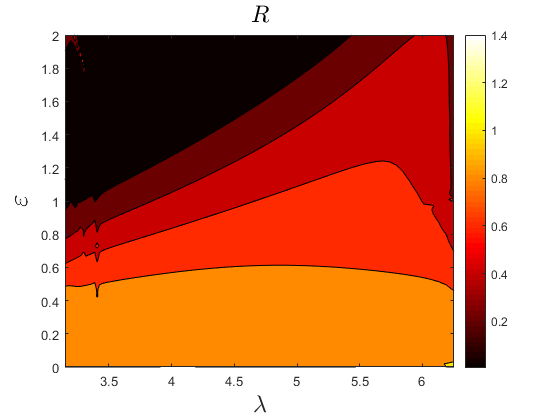
\includegraphics[width=7.6cm]{sections/6_scattering_and_reflectivity/refl_map_lipschitz.png} }}
    \subfloat[\centering Energy Defect]
    {{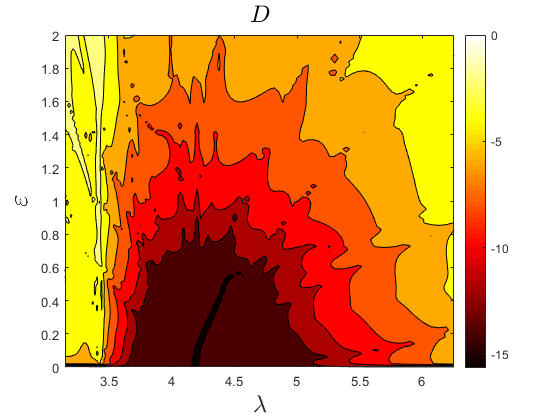
\includegraphics[width=7.6cm]{sections/6_scattering_and_reflectivity/energy_defect_lipschitz.png} }}
    \vspace{2mm}
    \caption{The Reflectivity Map, $R(\varepsilon,\delta)$, and Energy Defect $D$
    computed with Pad\'e summation. We set $N=M=20$ 
    with a granularity of $N_{\varepsilon}=N_{\delta}=100$ per invocation. (Top) The rough profile with grating surface, $(6.28)$, and physical parameters, $(6.30)$. (Bottom) The Lipschitz profile with grating surface, $(6.29)$, and physical parameters, $(6.30)$.}
    \label{Fig:RM:Single Case 2}
\end{figure}
